\paragraph{QuizziPedia::Front-End::Views::PasswordForgotView}
\begin{figure} [ht]
	\centering
	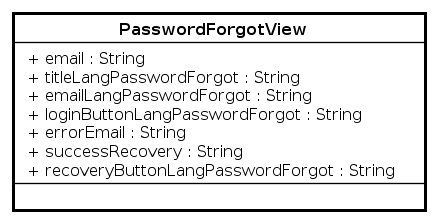
\includegraphics[scale=0.80]{UML/Classi/Front-End/QuizziPedia_Front-end_Views_PasswordForgotView.png}
	\caption{QuizziPedia::Front-End::Views::PasswordForgotView}
\end{figure} \FloatBarrier
\begin{itemize}
	\item \textbf{Descrizione}: view contenente le form necessarie per il recupero della password dimenticata;
	\item \textbf{Utilizzo}: permette all'utente di recuperare la password dimenticata inserendo i campi dati necessari;
	\item \textbf{Relazioni con altre classi}:
	\begin{itemize}
			\item \textit{IN} \texttt{PasswordForgotController}: questa classe permette di gestire il ripristino della password dimenticata;
			\item \textit{IN} \texttt{PasswordForgotModelView}: classe di tipo modelview la cui istanzazione è contenuta all'interno della variabile di ambiente \$scope di \texttt{Angular.js}. All'interno di essa sono presenti le variabili e i metodi necessari per il \textit{Two-Way Data-Binding\ped{G}} tra la view \texttt{PasswordForgotView} e il controller \texttt{PasswordForgotController};
			\item \textit{IN} \texttt{LangModel}: rappresenta il modello delle informazioni per la giusta traduzione dell'applicazione.
	\end{itemize}
	\item \textbf{Attributi}:
	\begin{itemize}
		\item \texttt{+ user: Object} \\ Campo dati contenente l'attributo \texttt{email};
		\item \texttt{+ titleLang: String} \\ Attributo che viene utilizzato per visualizzare la giusta traduzione del titolo della pagina, in italiano o in inglese;
		\item \texttt{+ emailLang: String} \\ Attributo che viene utilizzato per visualizzare la giusta traduzione della \textit{label\ped{G}} per l'inserimento della posta elettronica, in italiano o in inglese;
		\item \texttt{+ loginButtonLang: String} \\ Attributo che viene utilizzato per visualizzare la giusta traduzione della \textit{label\ped{G}} per il bottone di link all'autenticazione, in italiano o in inglese;
		\item \texttt{+ successRecovery: String} \\ Attributo che visualizza un messaggio di avvenuto invio della nuova password;
		\item \texttt{+ errorEmail: String} \\ Attributo che visualizza un eventuale messaggio di errore nell'inserimento della email.
	\end{itemize}
\end{itemize}